\documentclass[UTF8]{ctexart}
\usepackage{graphicx}
\graphicspath{{img/}} 
\title{Homework\ 2}
\author{PB17111623}
\author{PB17111623 范睿}
\date{\today}
\usepackage[a4paper,bottom=3.5cm]{geometry}
\usepackage{algorithm}  
\usepackage{algorithmicx}
\usepackage{amsmath}  
\usepackage{algpseudocode}  %算法的包
\usepackage{amssymb}
\begin{document}
\maketitle

\section{HW2}

\subsection{3.1-4}
$2^{n+1}=\mathcal{O}(2^{n})$成立\\
证明:\\
存在c=3,使得当n足够大时,$2^{n+1}=2*2^{n} \leq c2^{n}=3*2^{n}$均成立。\\
$2^{2n}=\mathcal{O}(2^{n})$不成立\\
证明:\\
${\forall}c \in \mathbb{R},{\exists}n_0 \in \mathbb{N},\emph{s.t.}\,$对于${\forall}n>n_0,$有$2^{n} \ge c,\,$即有$2^{2n} \ge c2^{n}$\\
所以不存在常数c满足上一条件,$2^{2n}=\mathcal{O}(2^{n})$不成立\\

\subsection{3.2-3}
证明$\lg(n!)=\Theta(n\lg n)$:\\
由斯特林近似公式:对于所有$n\ge 1$,有$n!=\sqrt{2\pi n}(\frac{n}{e})^{n}e^{\alpha_n}$,得:\\
$\lg(n!)=\lg(\sqrt{2\pi n}(\frac{n}{e})^{n}e^{\alpha_n})=\frac{1}{2}\lg(2\pi)+(n+\frac{1}{2})\lg(n)+(\alpha_n-n)lg(e)$\\
由$\frac{1}{12n+1}\le \alpha_n \le \frac{1}{12n}$ ,对于足够大的n,得\\
$\lg(n!)\leq (n+\frac{1}{2})\lg(n)+\frac{1}{12n}\lg(e) \le 2n\lg(n)$\\
$\lg(n!)\geq n(\lg(n)-\lg(e))) \ge \frac{1}{2}n\lg(n)$\\
∴存在$c_1=\frac{1}{2},c_2=2, \emph{s.t.}\,c_1n\lg(n) \leq \lg(n!) \leq c_2n\lg(n)$
命题得证

\subsection{4.3-2}
证明:\\
利用数学归纳法\\
①取$n_0>0, c_0>0$使得当$n\leq n_0$时,$T(n)<c\lg(n)$恒成立\\
②假设$T(\lceil\frac{n}{2}\rceil) \leq c\lg(\lceil\frac{n}{2}\rceil)$成立\\
③若$n$为偶数,有$T(\lceil\frac{n}{2}\rceil)\leq c\lg(n)-c\lg2$\\
$T(n)=T(\lceil\frac{n}{2}\rceil)+1 \leq c\lg(n)-c\lg2+1$\\
当$c \geq \frac{1}{\lg2}$时,$c\lg(n)-c\lg2+1 \leq c\lg(n)$,\\即有$T(n)\leq c\lg(n)$,其中$c \geq \frac{1}{\lg2}$\\\\
若n为奇数,有$T(\lceil\frac{n}{2}\rceil)\leq c\lg(n+1)-c\lg2$\\
$T(n)=T(\lceil\frac{n}{2}\rceil)+1 \leq c\lg(n+1)-c\lg2+1$\\
当$c \geq \frac{1}{\lg(\frac{2n}{n+1})}$时,$c\lg(n+1)-c\lg2+1 \leq c\lg(n)$,\\即有$T(n)\leq c\lg(n)$,其中$c \geq \frac{1}{\lg(\frac{2n}{n+1})}$\\\\
∴$\exists c \geq \max(c_0,\frac{1}{\lg2},\frac{1}{\lg(\frac{2n}{n+1})}), s.t.T(n)\leq c\lg(n)$\\命题得证

\subsection{4.4-8}
设$n=ta$\\
递归树如下:\\
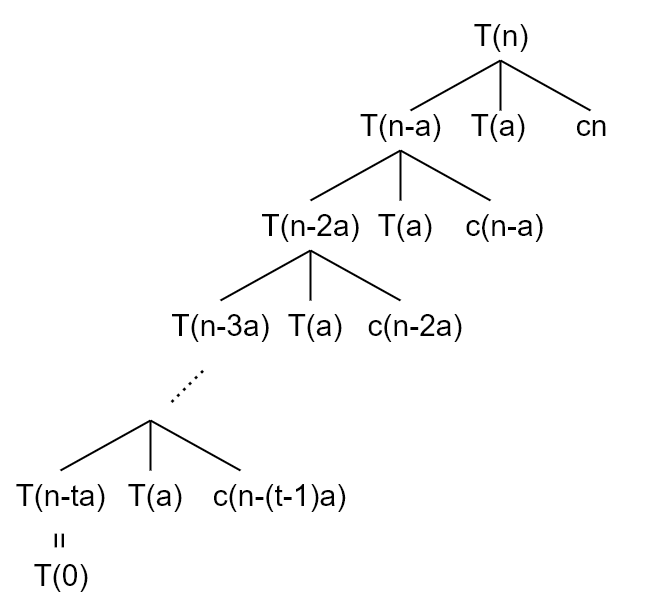
\includegraphics[scale=0.3]{44-8.png}
$\\T(n)=T(n-a)+T(a)+cn\\T(n-a)=T(n-2a)+T(a)+c(n-a)\\T(n-2a)=T(n-3a)+T(a)+c(n-2a)\\......\\T(n-(t-1)a)=T(n-ta)+T(a)+c(n-(t-1)a)=T(0)+T(a)+c(n-(t-1)a)\\$
∴$T(n)=T(0)+tT(a)+c(n+(n-a)+(n-2a)+...+(n-(t-1)a))\\=T(0)+tT(a)+ctn+\frac{t(t-1)}{2}ca$
\\又由$t=\frac{n}{a}$,得$T(n)=\frac{c}{2a}n^{2}+(\frac{T(a)}{a}+\frac{c}{2})n+T(0)$\\
解得$T(n)=\mathcal{O}(n^{2})$

\subsection{4.5-1}
\subsubsection{a.$T(n)=2T(\frac{n}{4})+1$}
$a=2,b=4,f(n)=1,n^{\log_ba-\epsilon}$$=n^{\log_42-\epsilon}$,$f(n)=\mathcal{O}(n^{\log_42-\epsilon})$\\
$T(n)=\Theta(\sqrt n)$
\subsubsection{b.$T(n)=2T(\frac{n}{4})+\sqrt n$}
$a=2,b=4,f(n)=\sqrt n,f(n)=\Theta(n^{\log_ba})\\ T(n)=\Theta(\sqrt n\lg n)$
\subsubsection{c.$T(n)=2T(\frac{n}{4})+n$} 
$a=2,b=4,f(n)=n,f(n)=\Omega(n^{\log_ba+\epsilon})$,且对于某个常数$c<1$和所有足够大的$n$有\\$2\frac{n}{b}\leq cf(n)$∴$T(n)=\Theta(n)$
\subsubsection{d.$T(n)=2T(\frac{n}{4})+n^{2}$}
$a=2,b=4,f(n)=n^{2},f(n)=\Omega(n^{\log_ba+\epsilon})$,且对于某个常数$c<1$和所有足够大的$n$有\\$2\frac{n}{b}\leq cf(n)$∴$T(n)=\Theta(n^{2})$

\subsection{4.5-4}
无法求解\\
证明:\\
$a=4,b=2,f(n)=n^2\lg n,n^{\log_ba}=n^{2}$,对于任意正常数$\epsilon$,比值$\frac{f(n)}{n^{\log_ba}}=\lg n$都渐进小于$n^{\epsilon}$,情况既不属于第二种又不属于第三种。
\\上界为$\mathcal{O}(n^{2}\lg n\log_2n)$
\end{document}
